\documentclass{beamer}
% \usepackage{animate}
\usepackage{multimedia}
\usepackage[english,russian]{babel}

\usepackage{pgfpages}
\setbeameroption{show notes on second screen}
%https://tug.ctan.org/macros/latex/contrib/beamer/doc/beameruserguide.pdf

\usepackage[T2A]{fontenc}
\usepackage[utf8]{inputenc}

\setbeamertemplate{caption}[numbered]

\usetheme{CambridgeUS}
\usecolortheme{dolphin}


\title[Введение в КГ]{Введение в компьютерную графику}
\author[Быковских Д.А.]{Быковских Дмитрий Александрович}
\date{06.09.2025}

\begin{document}
	\begin{frame}
		\titlepage

		\note{
			\begin{figure}
				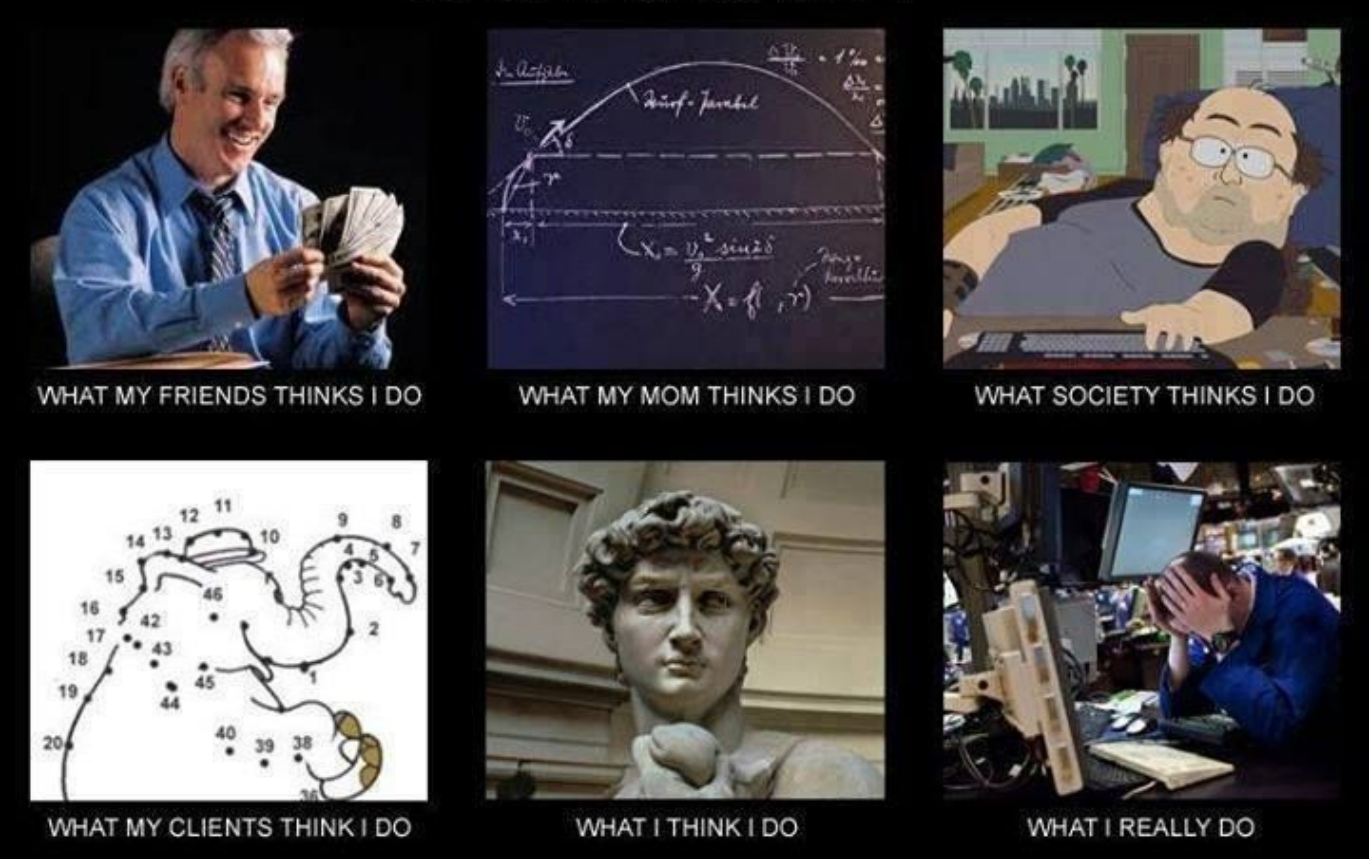
\includegraphics[width=0.8\textwidth]{images/cg_work_meme.png}
				\caption{Изображение для привлечения внимания}
			\end{figure}
		}
	\end{frame}
	%\section{Обзор}
	\begin{frame}{Содержание}
		\begin{itemize}
			\item 
			Общая информация о компьютерной графике
			\item
			Некоторые факты из истории компьютерной графики
			\item
			Аппаратные средства, связанные с выводом изображения
			\item 
			Терминология
		\end{itemize}
	\end{frame}
	\begin{frame}{Что такое компьютерная графика (КГ)?}
		Компьютерная графика --- междисциплинарная область информатики, изучающая математические и вычислительные основы генерации, обработки, представления и визуализации изображений и геометрической информации с использованием вычислительных систем.

		% Компьютерная графика --- одно из направлений информационных технологий, которое занимается созданием, редактированием и визуализацией \textbf{графических изображений}.
		{
			Спектр применений:
			\vskip-4mm
			\begin{columns}[t]
				\begin{column}{0.48\textwidth}
					{\footnotesize
						\begin{itemize}
							\item Разработка игр (виртуальный мир, персонажи, эффекты)
							\item Визуализация данных (диаграммы, графики)
							\item Дизайн (логотипы, баннеры, упаковки, интерфейсы)
							\item Симуляция и моделирование (виртуальные среды для тестирования)
						\end{itemize}
					}
				\end{column}
				\begin{column}{0.48\textwidth}
					{\footnotesize
						\begin{itemize}
							\item Анимация (фильмы, видеоролики, реклама)
							\item Медицинская визуализация (модели органов, тканей)
							\item Архитектурное проектирование (модели зданий, интерьеров)
							\item Редактирование фото и видео (улучшение качества)
							\item и многое другое
						\end{itemize}
					}
				\end{column}
			\end{columns}
		}
		\note{

		Машинная графика (Computer graphics, ГОСТ 27459-87) --- совокупность методов и приемов для преобразования при помощи ЭВМ данных в графическое представление или графического представления в данные.

		}
		
		\if 0
		3D-моделирование и анимация: Создание трехмерных моделей объектов, персонажей и сцен, а также их анимация для использования в фильмах, играх, визуализации архитектурных проектов и многих других областях.
		
		2D-графика и иллюстрации: Создание двумерных изображений, иллюстраций, рисунков, артов и графических элементов для книг, журналов, рекламы и дизайна.
		
		Визуализация данных: Преобразование сложных данных в наглядные и понятные визуальные формы, такие как графики, диаграммы, инфографика и карты.
		
		Компьютерная анимация и эффекты: Создание анимаций, спецэффектов и визуальных элементов для фильмов, рекламы, игр и других медийных продуктов.
		
		Графический дизайн: Разработка дизайна логотипов, брендинга, упаковки, веб-сайтов, приложений и других визуальных элементов.
		
		Виртуальная реальность (VR) и дополненная реальность (AR): Создание виртуальных и дополненных миров, в которых пользователи могут взаимодействовать и иметь визуальный опыт.
		
		Компьютерное моделирование: Создание компьютерных моделей и симуляций для изучения поведения систем, процессов и явлений в науке, инженерии и других областях.
		
		Медицинская визуализация: Создание графических изображений и моделей для обучения, диагностики и планирования медицинских процедур.
		
		Архитектурная визуализация: Создание виртуальных моделей зданий и помещений для архитекторов и дизайнеров.
		
		Ретушь и обработка фотографий: Использование графических инструментов для улучшения и изменения фотографий.
		
		Генеративное искусство: Использование алгоритмов и программирования для создания уникальных искусственных изображений и анимаций.
		\fi
		
	\end{frame}
	
	\begin{frame}{Основные направления}
		
		\begin{columns}
			\begin{column}{0.3\textwidth}
				
				\textbf{Image Processing}
				
				Image Compression
				
				Noise Reduction
				\begin{figure}
				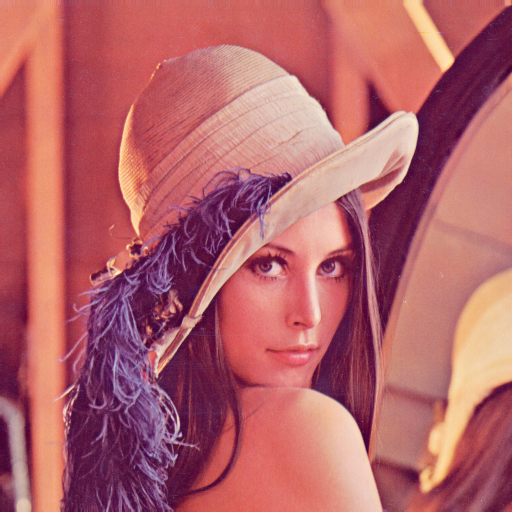
\includegraphics[width=\textwidth]{images/Lenna_test_image.png}
				\caption{Эталонное изображение (Söderberg Lenna)}
				\end{figure}
				
			\end{column}


			\begin{column}{0.3\textwidth}
				
				\textbf{Neural Networks}

				Computer Vision
				
				Machine Learning
				
				Deep Learning
				
				Data Mining				

				\vspace{2.5mm}

				\begin{figure}
				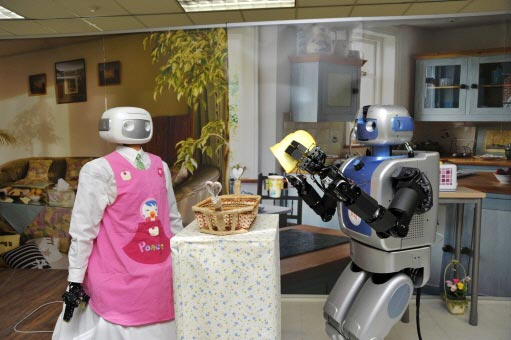
\includegraphics[width=\textwidth]{images/Computer_vision.png}
				\caption{Применение нейронных сетей (семейная пара)}
				\end{figure}
			\end{column}
			
			\begin{column}{0.4\textwidth}
				
				\textbf{Rendering}
				
				Computer-Generated Imagery
				
				RealTime Processing
				\begin{figure}
				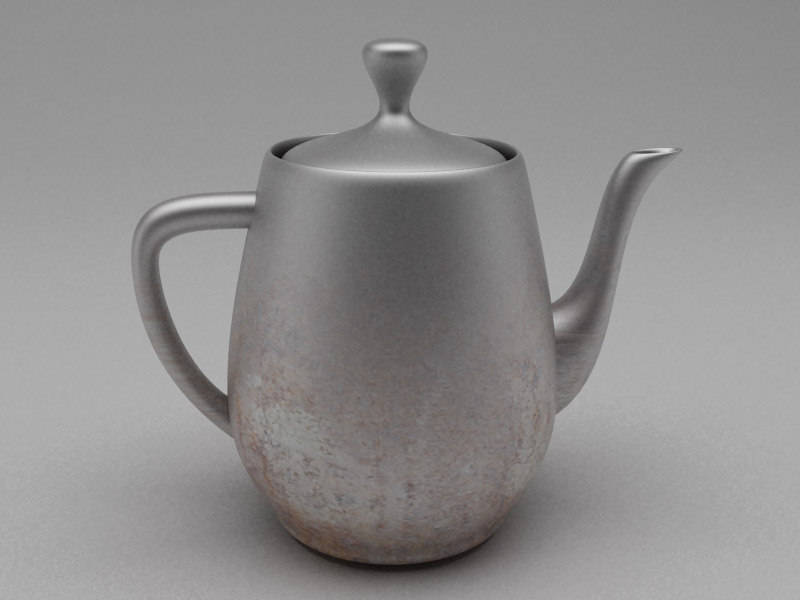
\includegraphics[width=\textwidth]{images/Utah_teapot.png}
				\caption{Классическая модель рендера (Newell teapot или чайник Юта)}
				\end{figure}
				
			\end{column}
		\end{columns}

		\note{
			Самые популярные направления на сегодняшний день: 
			\begin{itemize}
				\item рендеринг;
				\item анимация и симуляция;
				\item геометрическое моделирование;
				\item машинное обучение и ИИ;
				\item виртуальная и дополненная реальность;
				\item научная визуализация;
				\item вычислительная фотография. 
			\end{itemize}

		}

		\end{frame}
\if 0	
	\begin{frame}
	%https://iasl.uni-muenchen.de/links/GCA-IV.2e.html
	%https://www.timetoast.com/timelines/6248910a-e70f-4a32-b27c-e13ef9c355dc
	%https://web.archive.org/web/20070405181508/http://accad.osu.edu/\%7Ewaynec/history/lesson2.html
	%https://web.archive.org/web/20051103164835/http://accad.osu.edu/~waynec/history/lesson2.html
	

	История компьютерной графики насчитывает несколько десятилетий и прошла через ряд важных этапов и достижений. Вот краткий обзор этой истории:
	
	1950-е годы: Ранние исследования в области компьютерной графики начались в 1950-х годах. В 1950 году Иван Сазерленд (Ivan Sutherland) создал устройство "Скетчпад" (Sketchpad), позволяющее рисовать графику с помощью светового пера и дисплея.
	
	1960-е годы: В 1963 году Сазерленд представил прототип первого компьютерного графического устройства для рисования 3D-изображений, названного "TX-2 Sketchpad". Этот момент считается началом трехмерной компьютерной графики.
	
	1970-е годы: В 1970-х годах были разработаны первые программы для создания и редактирования графики, такие как "SuperPaint" и "Computer Graphics System" на основе аппаратных решений. Были также созданы первые алгоритмы заполнения и отсечения для растровой графики.
	
	1980-е годы: В это десятилетие произошли значительные прорывы в компьютерной графике. Были разработаны первые графические интерфейсы пользователя (GUI), например, интерфейс для компьютера Apple Macintosh. Также были созданы первые 3D-моделирование и анимационные программы.
	
	1990-е годы: С распространением персональных компьютеров и улучшением аппаратного обеспечения появились новые возможности для компьютерной графики. Были разработаны 3D-игры, программы для редактирования фотографий и видеороликов.
	
	2000-е годы: Развитие 3D-графики продолжилось, и стали доступны более мощные инструменты для создания сложных 3D-моделей и анимаций. Также стали популярными виртуальная и дополненная реальность.
	
	2010-е годы: Продолжалось усовершенствование компьютерной графики, включая разработку более реалистичных графических движков для видеоигр, прорывы в области визуализации данных и рост популярности анимации и цифрового искусства.
	
	\end{frame}
\fi
	
	\section{История развития. Интересные факты}
	
	\begin{frame}{Spacewar (1962 г.)}{Одна из первых компьютерных игр}
	
	\begin{columns}
		
		\begin{column}{0.5\textwidth}
			
			%Название: Spacewar!
			
			\textbf{Жанр:} Shoot’em up, космический симулятор
			
			\textbf{Авторы:} Steve Russell, Martin Graetz, Wayne Wiitanen, Bob Saunders, Steve Piner
			
			\textbf{Платформа:} DEC PDP-1
			
			\textbf{Время разработки:} 200 чч
			
		\end{column}
		\begin{column}{0.5\textwidth}
			\begin{figure} 
			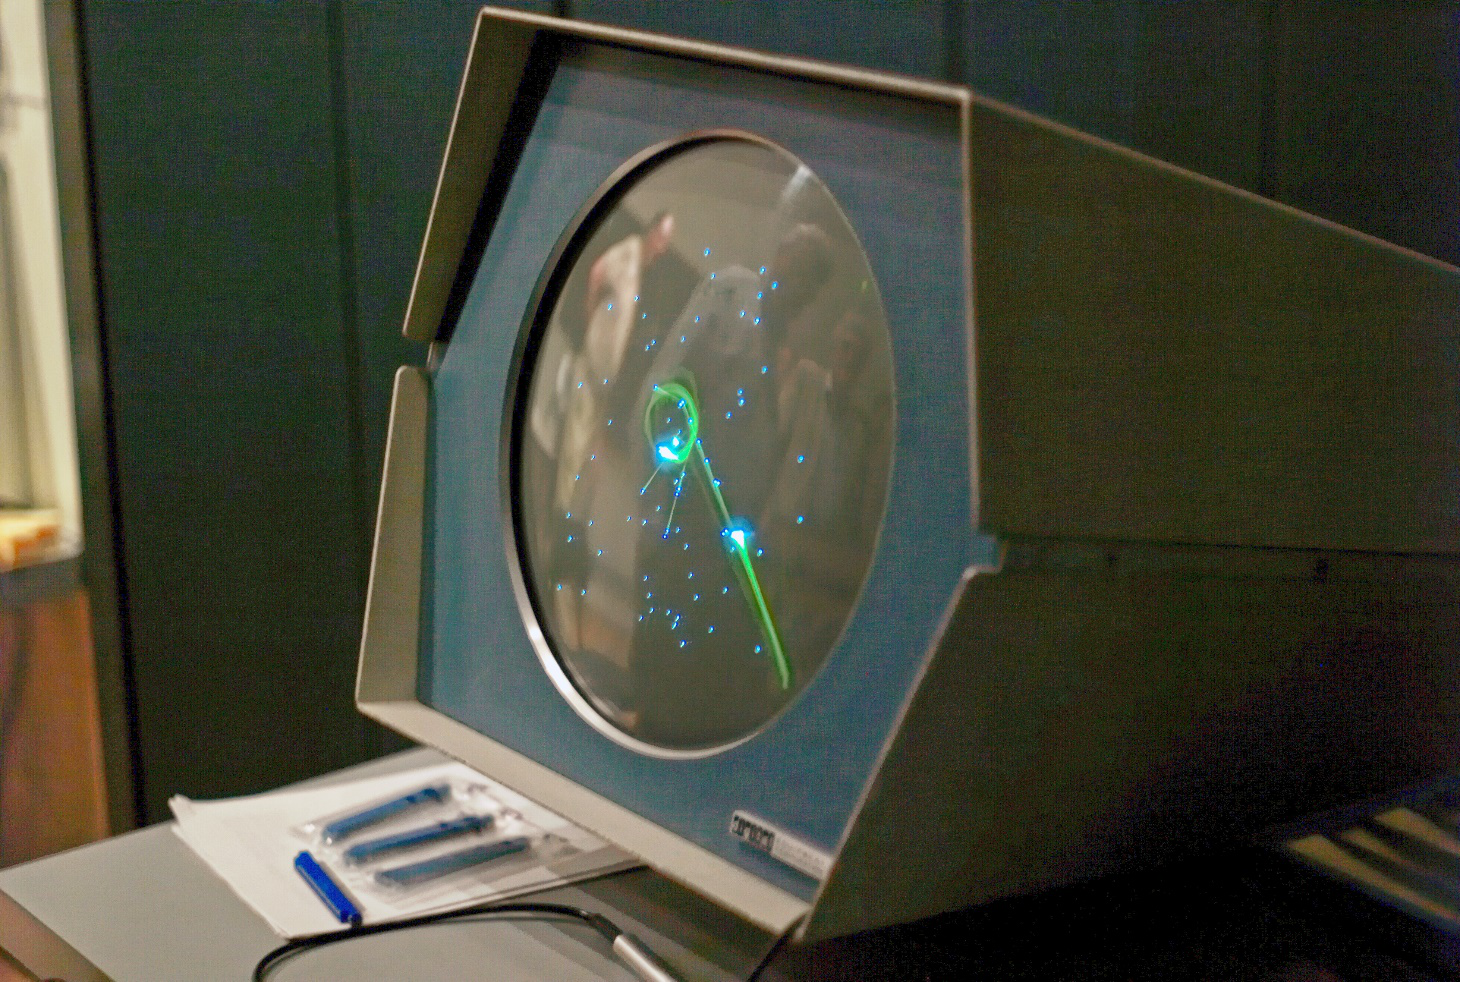
\includegraphics[width=\textwidth]{images/Spacewar.png}
			\caption {DEC PDP-1 and Spacewar}
			\end{figure}
		\end{column}
		
	\end{columns}
	
	\note{
		ЭЛТ (Электронно-лучевая трубка)
		
		Работает с помощью электронного пучка, испускаемого анодом и фосфорного экрана, выполняющего роль катода. 
		Имеет крупные размеры, высокое энергопотребление и вес, но обеспечивает хорошее качество изображения и высокую частоту обновления.
		
		% LCD (Liquid Crystal Display или жидкокристаллический дисплей)
		
		% Основан на управлении светом через жидкие кристаллы с подсветкой. Более тонкий, легкий, с меньшим энергопотреблением, но может иметь ограничения по углам обзора и контрасту.
		
		% OLED (Organic Light-Emitting Diode или органический светодиод)
		
		% Использует органические светодиоды для создания изображения. Тонкий, энергоэффективный, обеспечивает отличное качество изображения, особенно в темных сценах, но может быть подвержен эффекту выгорания пикселей (особенно на статичных изображениях).
	}
	
	\end{frame}

\begin{frame}{Кошечка (1968 г.)}{Одна из первых компьютерных анимаций}
	
	\begin{columns}
		\begin{column}{0.5\textwidth}
			
			\textbf{Авторы:} Н.Н. Константинов, В. Минахин, В. Понамаренко, А. Скуридин, В. Журкин
			
			\textbf{Платформа:} БЭСМ-4 и алфавитно-цифровой принтер
			
			\textbf{Реализация:} движения кошки описаны дифференциальными уравнениями
			
		\end{column}
		\begin{column}{0.5\textwidth}
			\begin{figure}
				\href{https://www.youtube.com/watch?v=LzMk5sC6eAU}{
				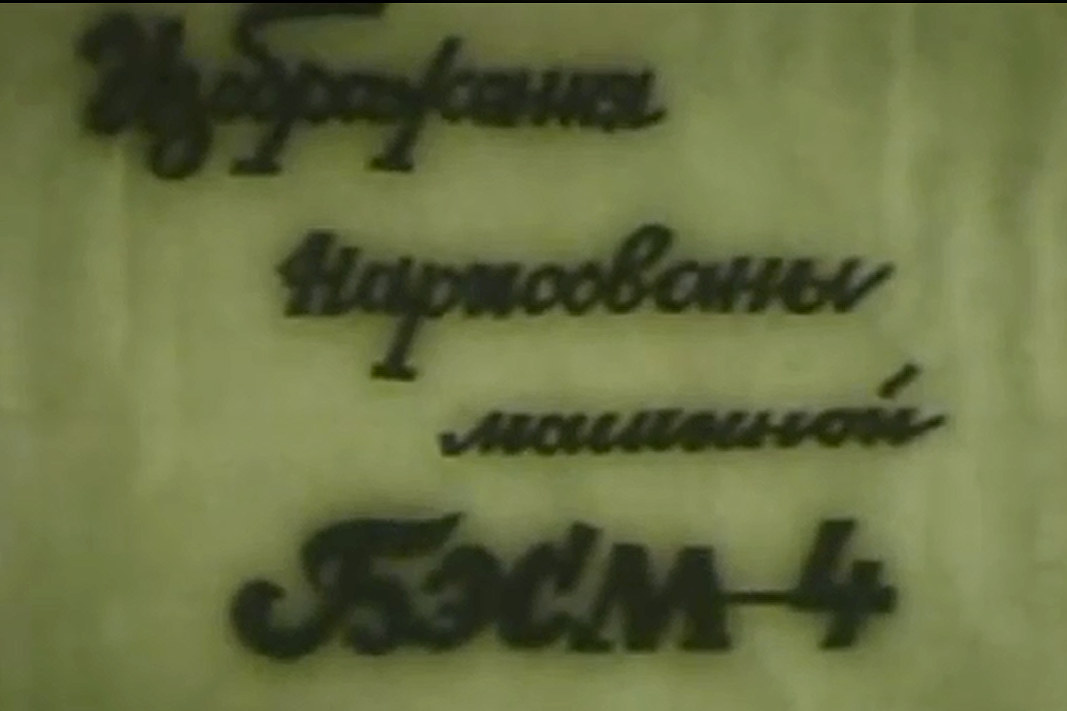
\includegraphics[width=\textwidth]{images/AnimatedCat.jpg}
				}
				\caption {Кошечка}
			\end{figure}
		\end{column}
	\end{columns}
\end{frame}

\begin{frame}{Чайник Юта (1975 г.)}{Newell teapot}
	\begin{columns}
		\begin{column}{0.5\textwidth}
			\begin{figure} 
				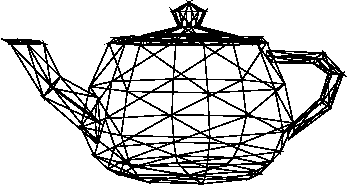
\includegraphics[width=\textwidth]{images/Utah_teapot_model.png}
				\caption {Состоит из 32 кубических поверхностей Безье}
			\end{figure}
		\end{column}
		\begin{column}{0.5\textwidth}
			\begin{figure} 
				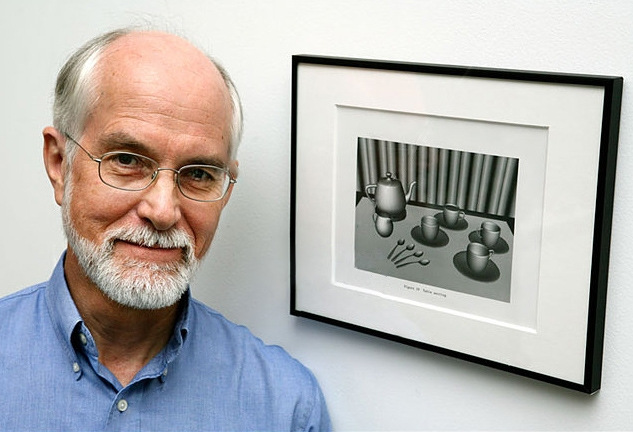
\includegraphics[width=\textwidth]{images/Utah_teapot_and_Newell.png}
				\caption {Мартин Ньювелл и чайник Юта}
			\end{figure}
		\end{column}
	\end{columns}

	\note{
		https://www.opengl.org/resources/libraries/glut/spec3/node89.html
		
		Скомпилировать программу из 
		CG/Projects/src/utah\_teapot.c
	}

\end{frame}

\begin{frame}{Silicon Graphics Inc. (SGI, 1982 г.)}{}
	\begin{columns}
		\begin{column}{0.5\textwidth}
			
			\textbf{Описание:} Разработка графических станций (Indigo, Indy и др.) и ПО (SGI IRIX и др.) для визуализации
			
			\textbf{Основатель:} Джим Кларк
			
		\end{column}
		\begin{column}{0.5\textwidth}
			\begin{figure} 
				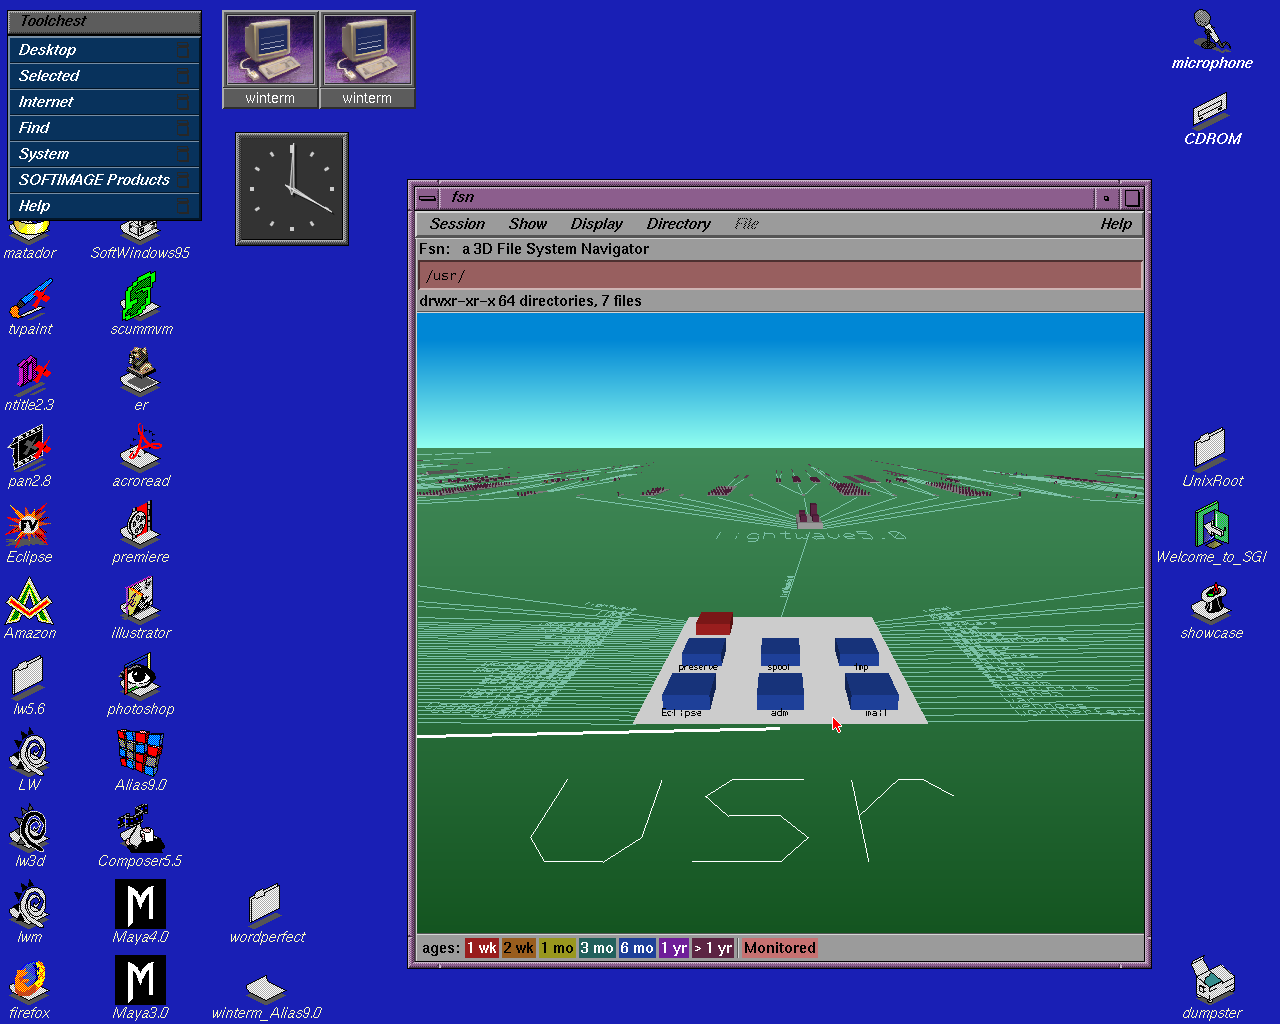
\includegraphics[width=\textwidth]{images/IRIX_OS.png}
				\caption {IRIX OS}
			\end{figure}
		\end{column}
	\end{columns}
	\note{
		История компании Silicon Graphics

	https://habr.com/ru/companies/vdsina/articles/562912/	

	{
	\scriptsize

		В 1984 году SGI выпустила системы IRIS первого поколения (модели 1000 и 1200).

		Вскоре получила статус легенды среди 3D-художников и графических дизайнеров, использовавших уникальную мощь её рабочих станций.

		Наследие можно увидеть в Nintendo 64 (вышла в 1996 г.). 
		
		Принимала участие в разработке голливудских фильмов, включая 
		Jurassic Park, «Парк юрского периода» (1993 г.),
		Jumanji, «Джуманджи» (1995 г.),
		The Matrix, «Матрица» (1999 г.),
		Star Wars. Episode I, «Звёздные войны. Эпизод I» (1999 г.),
		Lord of the Rings, «Властелин колец» (2000 г.),
		и другие.

		В 1992 году SGI решили перепроектировать API и начали продавать недорогие лицензии на него своим конкурентам.
		После SGI организовала OpenGL Architecture Review Board для руководства дальнейшими разработками.

		В феврале 1996 года SGI решила войти на рынок суперкомпьютеров, приобретя за 740 миллионов долларов Cray Research.

		В 2003 году компания освободила помещения своей штаб-квартиры в Маунти-Вью и сдала здание в аренду Google.

		В апреле 2009 года снова SGI подала заявку согласно Главе 11 и была продана Rackable Systems за 25 миллионов.
		
		\_
		
		}
	}

\end{frame}


\begin{frame}{Первая 3D видеокарта (1996 г.)}{}
	\begin{columns}
		\begin{column}{0.5\textwidth}
			
			\begin{figure}
				\href{https://www.youtube.com/watch?app=desktop&v=Zdf270cZD9g}{
				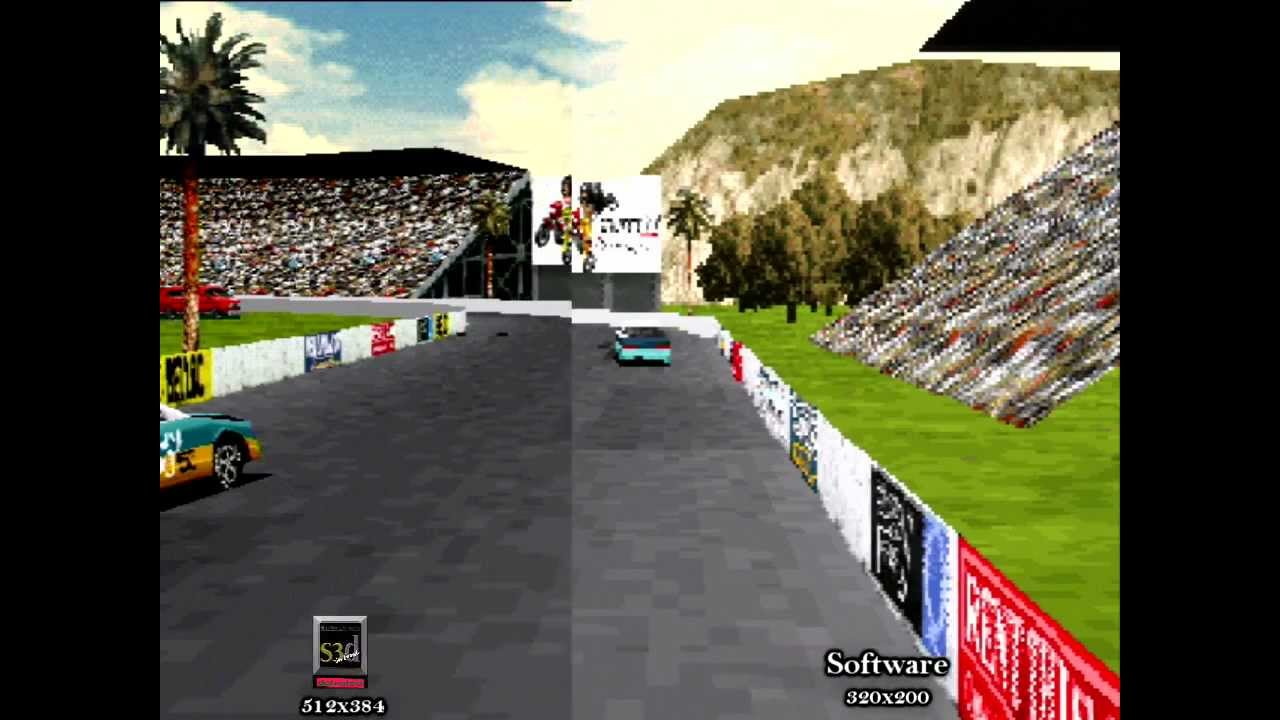
\includegraphics[width=\textwidth]{images/Destruction_Derby_1995.png}}
				\caption {Destruction Derby (1995 г.)}
			\end{figure}
		\end{column}
		\begin{column}{0.5\textwidth}
			\begin{figure} 
				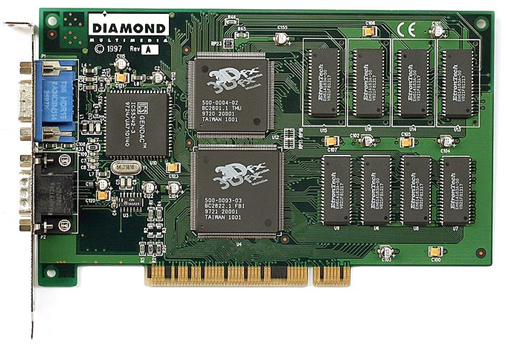
\includegraphics[width=\textwidth]{images/Diamond_Monster_3D_3DFX_Voodoo1.png}
				\caption {Diamond Monster 3DFX Voodoo1}
			\end{figure}
		\end{column}
	\end{columns}
\end{frame}

\section{Аппаратные средства}

\begin{frame}{Характеристики видеокарты 3DFX Voodoo1}{1996 г.}
	\begin{columns}
		\begin{column}{0.5\textwidth}
			\textbf{Разработчик:} Diamond
			
			\textbf{Шины I/O:} PCI/VGA
			
			\textbf{Память:} 4 MB EDO DRAM
			
			\textbf{Тех процесс:} 500 nm
			
			\textbf{Частота min/max:} 45/50 MHz
			
			\textbf{API:}  DX5 (DirectX 5)
			
			\textbf{Цена:} 300\$
			
			\textbf{Эффекты:} texture modulation, Z-buffering, Bi-linear texture filtering, anti-aliasing etc.
		\end{column}
		\begin{column}{0.5\textwidth}
			\begin{figure} 
				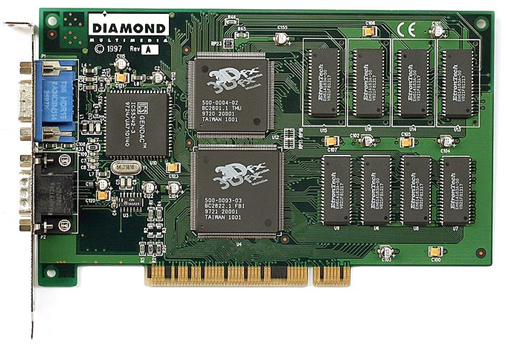
\includegraphics[width=\textwidth]{images/Diamond_Monster_3D_3DFX_Voodoo1.png}
				\caption {Diamond Monster 3DFX Voodoo1}
			\end{figure}
			
		\end{column}
	\end{columns}
\note{
{\tiny
	\begin{enumerate}
		\item	
	\textbf{Texture Modulation (текстурная модуляция)} \\
	- это техника в компьютерной графике, которая позволяет комбинировать две или более текстуры в одной точке на поверхности объекта. Это достигается путем умножения цветов пикселей из различных текстур и последующим объединением результатов. Это может использоваться для создания сложных визуальных эффектов, таких как освещение, тени и детализация.
	
	\item
	\textbf{Z-buffering (Буфер глубины)} \\
	- это метод решения проблемы видимости в трехмерной графике. Он использует буфер глубины (или Z-буфер), который хранит информацию о расстоянии от камеры до каждого пикселя на экране. Во время рендеринга сцены каждый новый пиксель сравнивается с содержимым Z-буфера. Если новый пиксель ближе к камере, его глубина записывается в Z-буфер, и цвет пикселя рендерится на экране. Это обеспечивает правильное наложение объектов в сцене и решает проблему перекрытия.
	
	\item
	\textbf{Bi-linear Texture Filtering (Билинейная фильтрация текстуры) } \\
	- это метод интерполяции цветов пикселей на текстуре для сглаживания артефактов, таких как лестничные эффекты или пиксельные артефакты, которые могут возникнуть при растягивании или сжатии текстур. Для каждого пикселя на экране берутся ближайшие четыре пикселя на текстуре, и их цвета интерполируются на основе расстояния до центра пикселя на экране. Это обеспечивает более плавное и реалистичное отображение текстур на объектах.
	\item
	\textbf{Anti-aliasing (Сглаживание краев)} \\
	- это техника, которая используется для смягчения ступенчатых краев (лестничных эффектов) на объектах или линиях в компьютерной графике. Она достигается путем усреднения цветов пикселей, находящихся на границе объекта, с окружающими пикселями. Это создает плавный переход цветов и уменьшает эффект "мерцания" на границах объектов при их движении или вращении.
\end{enumerate}
}
}
\end{frame}


\begin{frame}{Характеристики видеокарты}{Графический процессор (видеочип)}
	Число транзисторов, млрд.
	
	Техпроцесс, нм
	
	Тактовая частота, ГГц
	
	Количество шейдерных ядер (ALU, Arithmetic Logic Unit)
	
	Тензорные ядра (Tensor Cores)

	RT-ядра (Ray-Tracing Cores)

	Скорость заполнения (Fill Rate)
	\begin{itemize}
		\item 
		Пиксельная – число блоков растровых операций (Raster Operations Pipeline
	or Render Output Unit, ROPs)
		\item 
		Текстурная – количество блоков наложения текстур (Texture Mapping Unit,
		TMUs)
	\end{itemize}
	
	
	\note{
	
		Описание самой мощной игровой видеокарты на 2025 г. NVIDIA GeForce RTX 5090

		https://www.techpowerup.com/gpu-specs/geforce-rtx-5090.c4216

		С различными характеристиками можно ознакомиться:

		https://www.thg.ru/graphic/graphic\_card\_faq\_ii/index.html
		
		\tiny
		{\small
		Скорость заполнения (Fill Rate)
		}
	
		С какой скоростью графический процессор может выдавать пиксели (например, triangle fill rate у старых видеокарт). 
		Выделяют два типа скорости заполнения: пиксельную (pixel fill rate, ${PFR = ROP \cdot Hz}$) и текстурную (texture fill rate).

		Текстурную скорость заполнения ATi и nVidia считают по-разному. nVidia считает, что скорость получается умножением числа пиксельных конвейеров на тактовую частоту. А ATi умножает число текстурных блоков на тактовую частоту. В принципе, оба способа корректны, поскольку nVidia использует по одному текстурному блоку на блок пиксельных шейдеров, т.е. по одному на пиксельный конвейер.

		{\small
		Блоки наложения текстур (Texture Mapping Unit, TMU)
		}

		Текстуры следует выбрать и отфильтровать. Эта работа выполняется блоками наложения текстур, которые работают совместно с блоками пиксельных и вершинных шейдеров. 
		Работа TMU заключается в применении текстурных операций над пикселями.

		{\small
		Блоки растровых операций (Raster Operations Pipeline, ROP)
		}

		Процессоры растровых операций отвечают за запись пиксельных данных в память. Скорость, с которой выполняется эта операция, является скоростью заполнения (fill rate). 
		Производительность (и число) ROP уже редко используется для оценки скорости видеокарты, т.к. перестала быть узким местом. 

		\_
	}
	
\end{frame}

\begin{frame}{Характеристики видеокарты}{Графическая память и прочие атрибуты}
	\begin{columns}
		\begin{column}{0.5\textwidth}

			\textbf{Графическая память}
			
			Разрядность шины, бит
			
			Тип микросхем (GDDR5X SDRAM)
			
			Тактовая частота, ГГц
			
			Объем, Tбайт

			\vspace{25mm}
		\end{column}
		\begin{column}{0.5\textwidth}
			\textbf{Другие атрибуты}
			
			Размеры
			
			Тип охлаждения
			
			Шина I/O (PCIe)
			
			Мощность, Вт (Энерговыделение)
			
			Производительность шейдерных  ALU (FP32/FP64/FP16)
			\begin{itemize}
				\item 
				Бенчмарки (benchmark)
				\item 
				Тесты на играх
			\end{itemize}
			
		\end{column}
	\end{columns}
\end{frame}


\begin{frame}{ Характеристики видеокарты}{Memory Hierarchy and Floating Point (FP)}
	\begin{figure}
		\href{https://www.researchgate.net/profile/M-Clark/publication/51927898/figure/fig4/AS:668607537233921@1536419867027/A-schematic-of-the-memory-hierarchy-of-the-Nvidia-Fermi-architecture-with-the-peak.png}{
			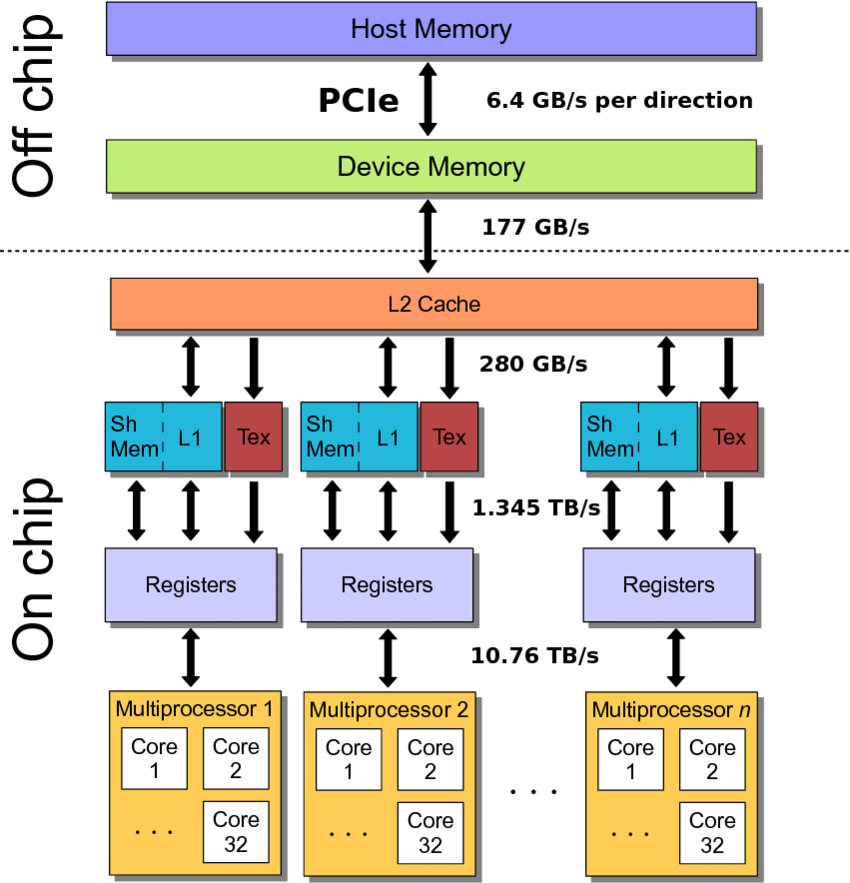
\includegraphics[width=0.5\textwidth]{images/Nvidia_Fermi_architecture_memory.png}}
		\caption {Nvidia Fermi Architecture Memory}
	\end{figure}
	
	\note{
	\begin{figure} 
		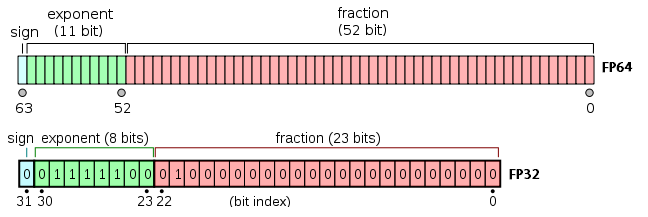
\includegraphics[width=\textwidth]{images/Floating_Point_structure.png}
		\caption {Структура чисел с плавающей точкой}
	\end{figure}
	}
\end{frame}

\begin{frame}{Характеристики видеокарты}{Бенчмарки (benchmark)} 
	\begin{figure} 
		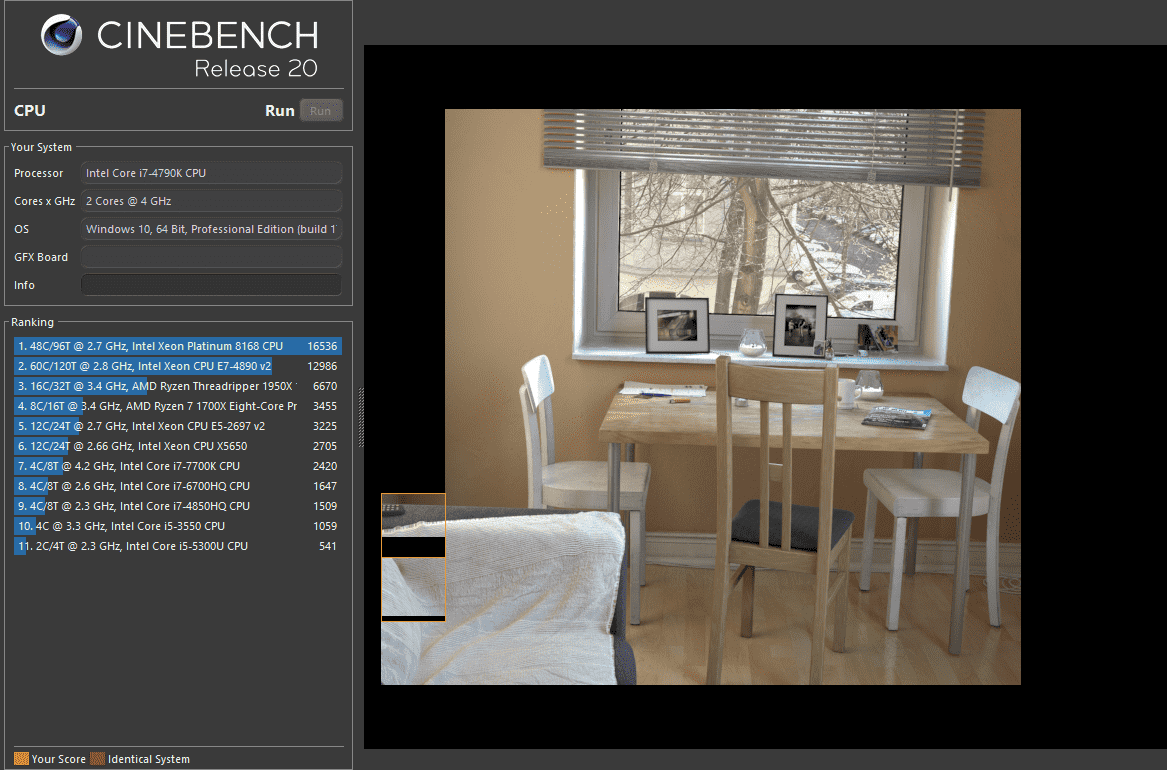
\includegraphics[width=0.8\textwidth]{images/Cinebench.png}
		\caption {Cinebench R23}
	\end{figure}
	
	\note{
		https://youtu.be/-bab7HjoZqk?si=HF1GxvNNv3mtCaRG
	
	Популярные
		\begin{itemize}
		\item 
		Cinebench R23
		\item 
		Furmark
		\item 
		3DMark
		\item 
		Heaven
		
	\end{itemize}
	
	и др.
	}

\end{frame}

\section{Программные средства}
\begin{frame}{Терминология}
	{\scriptsize
	
	\textbf{Спецификация (стандарт)} --- документированные наборы правил, рекомендаций и параметров, определяющие способы взаимодействия, описание, единое понимание и совместимость между аппаратной и программной частями.
	
	\textbf{Драйвер (видеодрайвер)} --- программный интерфейс между операционной системой и графическим аппаратным обеспечением компьютера или устройства. 
	%Графический драйвер выполняет важную роль в управлении и координации графическими функциями, такими как отображение изображений, обработка графики и управление монитором. Он обеспечивает абстракцию между аппаратурой и приложениями, позволяя программам использовать графические возможности устройства без необходимости знания специфических деталей аппаратной реализации.
	
	\textbf{Графическая библиотека} --- набор программных инструментов, функций и ресурсов, предназначенных для упрощения создания графических элементов в компьютерных приложениях. 
	%Графические библиотеки предоставляют разработчикам доступ к базовым операциям рисования, управлению окнами, обработке ввода и другим визуальным компонентам.
	
	\textbf{Графический фреймворк} --- комплексная структура, предоставляющая базовую архитектуру и инструменты для разработки графических приложений. 
	%В отличие от графических библиотек, фреймворки предоставляют более высокоуровневую абстракцию, объединяя не только графические, но и другие компоненты, такие как управление событиями, многозадачность и др.
	
	\textbf{Графический движок} --- программное обеспечение, которое предоставляет инфраструктуру и инструменты для разработки интерактивных графических приложений, игр и визуальных симуляций. 
	%Графические движки обычно включают в себя готовые решения для управления графикой, физикой, анимацией, освещением и другими аспектами визуализации.
	
	\textbf{Графические редакторы} --- программное обеспечение, предназначенное для создания, редактирования и манипулирования графическими изображениями, включая различные эффекты, анимацию и многое другое. 
	%Графические редакторы могут быть ориентированы на векторную или растровую графику, обеспечивая пользователю инструменты для рисования, изменения цветов, добавления эффектов и других операций над изображением.
	
	\textbf{Графический профилировщик} --- программное обеспечение, используемое для анализа и оптимизации производительности графических приложений или систем. 
	%Графический профилировщик собирает данные о времени выполнения, использовании ресурсов (например, CPU и GPU), вызовах функций и других аспектах работы с графикой. Эти данные помогают разработчикам и инженерам идентифицировать узкие места, проблемы с производительностью и оптимизировать код или конфигурацию, чтобы обеспечить более плавное и эффективное взаимодействие графических приложений с аппаратурой и операционной системой.
	
	\textbf{GPU benchmark (бенчмарк графического процессора)} --- методика тестирования и оценки производительности графического процессора, которая позволяет измерить его способность обрабатывать графику и выполнение вычислительных задач. 
	%В ходе GPU бенчмарка используются специально разработанные тестовые сцены или наборы задач, которые загружают графический процессор различными видами нагрузки, включая визуализацию 3D-графики, обработку текстур, вычисления с плавающей точкой и другие графические задачи. Результаты бенчмарка позволяют оценить производительность GPU, сравнить его с другими моделями или системами, а также определить, какие виды задач выполняются наиболее эффективно, что может быть полезно при выборе аппаратного обеспечения для конкретных целей.
}
\end{frame}

\if 0
\begin{columns}
	
	\begin{column}{0.5\textwidth}
		\begin{itemize}
			\item
			
		\end{itemize}
	\end{column}
	\begin{column}{0.5\textwidth}
		\begin{itemize}
			\item
		\end{itemize}
	\end{column}
	
\end{columns}
\fi
	
\end{document}
